\documentclass[tikz,border=10pt]{standalone}
\usetikzlibrary{shapes.geometric, positioning, arrows.meta, scopes, patterns, shadows, calc}
\usepackage{xstring}

\def\code#1{\color{olive}{\texttt{#1}}\color{black}~}
% \def\refer#1{Fig. \ref{#1}}
% \newcommand{\urlpath}[1]{%
% \begin{FVerbatim}[fontsize=\scriptsize]
% #1
% \end{FVerbatim}%
% }

\def\comment#1{\color{olive}{\textit{\% #1}} \color{black}}

\newcommand\ezeq[1]{$#1$}

\newcommand\ezcolumn[3]{
\begin{column}{#1\textwidth}
    \vspace{#2cm}
    #3
\end{column}
}

% \newenvironment{myenumerate}{%
%   \begin{enumerate}
%     \renewcommand{\theenumii}{\arabic{enumi}.\arabic{enumii}}
%   }
%   {%
%   \end{enumerate}
% }


\newcommand{\customenumerate}{%
  \renewcommand{\theenumii}{\arabic{enumi}.\arabic{enumii}}
  \renewcommand{\theenumiii}{\arabic{enumi}.\arabic{enumii}.\arabic{enumiii}}
}


\begin{document}
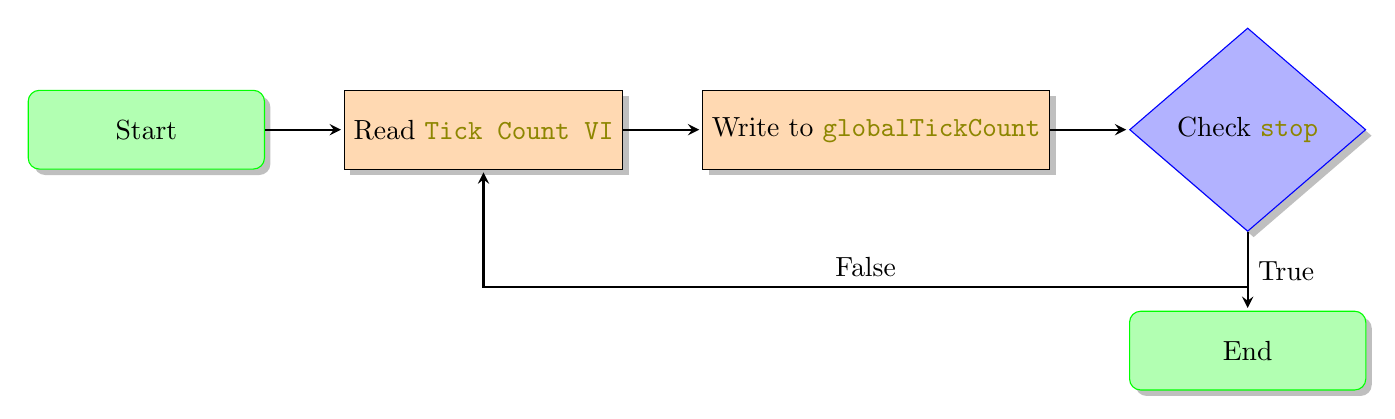
\begin{tikzpicture}[
    startstop/.style={rectangle, rounded corners, minimum width=3cm, minimum height=1cm, text centered, draw=green, fill=green!30, drop shadow},
    process/.style={rectangle, minimum width=3cm, minimum height=1cm, text centered, draw=black, fill=orange!30, drop shadow},
    io/.style={trapezium, trapezium left angle=70, trapezium right angle=110, minimum width=3cm, minimum height=1cm, text centered, draw=blue, fill=blue!30, drop shadow},
    decision/.style={diamond, minimum width=3cm, minimum height=1.5cm, text centered, draw=blue, fill=blue!30, drop shadow},
    arrow/.style={thick,->,>=stealth, shorten >=1pt},
]

% Start block
\node[startstop] (start) {Start};

% Process of getting tick count
\node[process, right=of start] (tick) {Read \code{Tick Count VI}};

% Process of writing tick count to globalTickCount
\node[process, right=of tick] (write) {Write to \code{globalTickCount}};

% Decision to continue or stop
\node[decision, right=of write] (decide) {Check \code{stop}};

% End block
\node[startstop, below=of decide] (end) {End};

% Draw the arrows
\draw[arrow] (start) -- (tick);
\draw[arrow] (tick) -- (write);
\draw[arrow] (write) -- (decide);
\draw[arrow] (decide) -- ++(0,-2cm) -|node[anchor=south, pos=0.25] {False} (tick);
\draw[arrow] (decide) -- node[anchor=west] {True} (end);

\end{tikzpicture}
\end{document}
